In this chapter, we analyze the fifth experiment group, that is, the impact of having different degrees of privacy, per scoring technique, in a Blockchain-based Federated Learning system. In this set of experiments, all properties of the system are static, except for the degree of privacy, which varies between 0, 1 and 5, per each scoring mechanism.

\section{Execution Time, Transaction Cost and Latency}

On \autoref{fig:priv_metrics}, we show the metrics regarding the execution time and transaction cost and latency per privacy degree for each of the scoring techniques.

As we can see per the figure, adding a privacy mechanism increases each round time by approximately $16.6$ seconds. From this 16.6 seconds, 10 seconds directly caused by the differential privacy mechanism. The remaining are caused by slight fluctuations on communication time, such as waiting for all devices to submit their updates after applying the differential privacy. Therefore, we can conclude that there is a trade-off between execution time and privacy level. However, the privacy degree does not seem to influence the execution time significantly.

Regarding transaction latency and costs, having a privacy mechanism or not in place does not create significant changes. This is expected since the communications with the blockchain remain the same whether or not the clients apply a differential privacy mechanism to their weights or not. 

\begin{figure}[!hpt]
    \centering
    \begin{subfigure}[b]{0.47\textwidth}
        \centering
        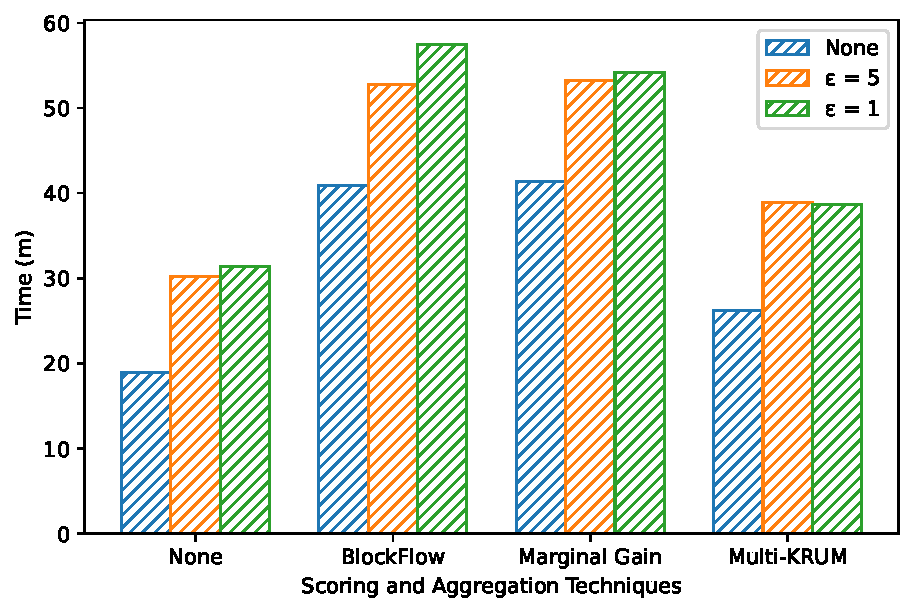
\includegraphics[width=\textwidth]{graphics/privacy/e2e.pdf}
        \caption{E2E Time}
    \end{subfigure}
    \hfill
    \begin{subfigure}[b]{0.47\textwidth}
        \centering
        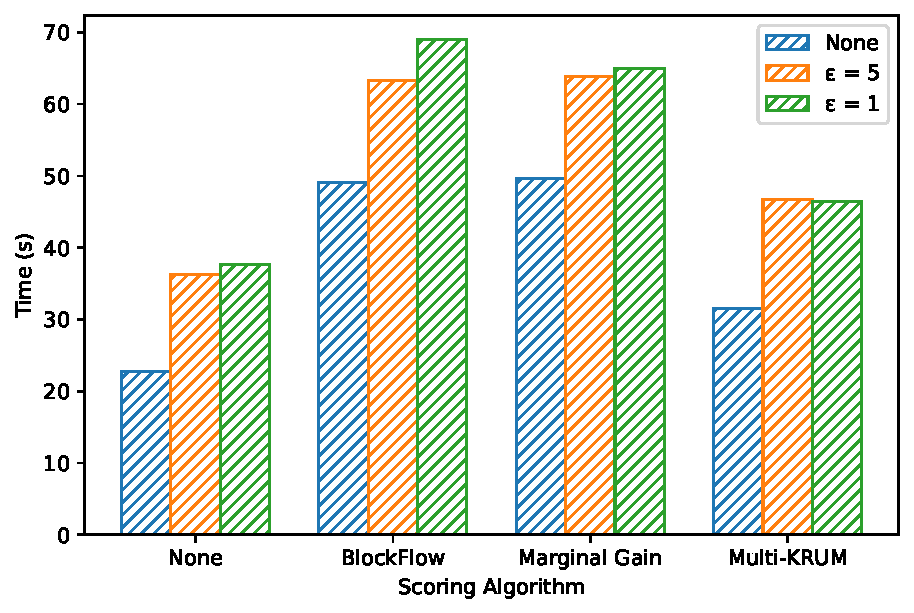
\includegraphics[width=\textwidth]{graphics/privacy/round.pdf}
        \caption{Mean Round Time}
    \end{subfigure}
    \hfill
    \begin{subfigure}[b]{0.47\textwidth}
        \centering
        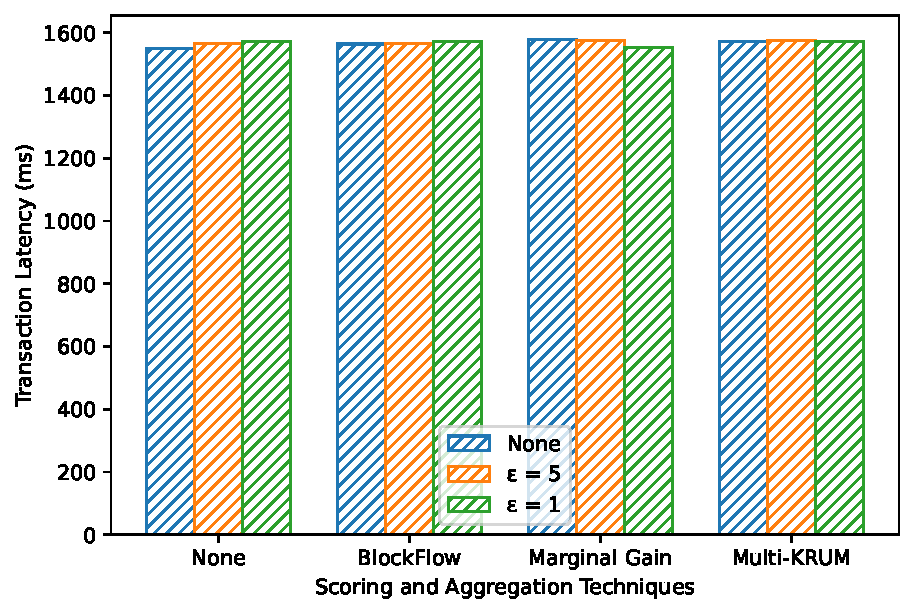
\includegraphics[width=\textwidth]{graphics/privacy/tx_latency.pdf}
        \caption{Transaction Latency}
    \end{subfigure}
    \hfill
    \begin{subfigure}[b]{0.47\textwidth}
        \centering
        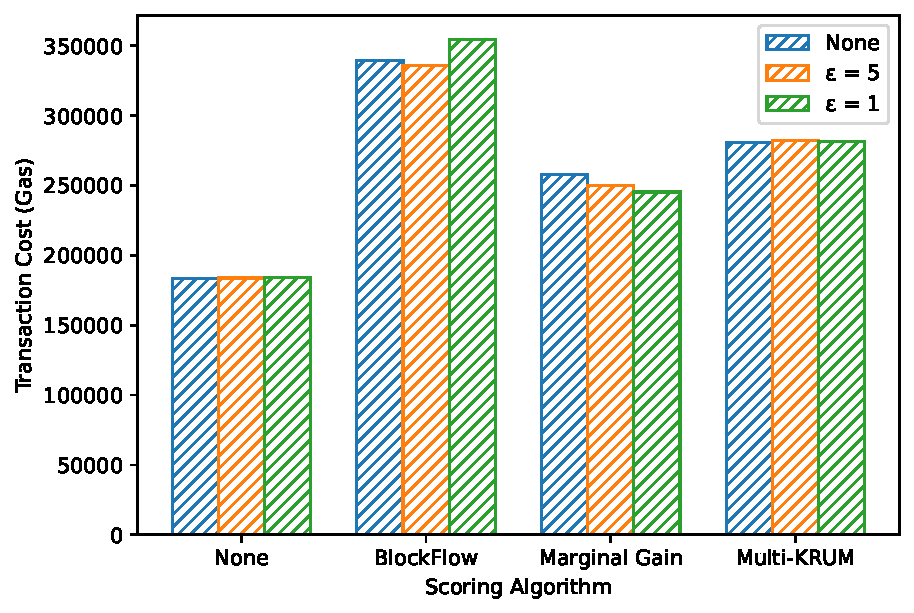
\includegraphics[width=\textwidth]{graphics/privacy/tx_cost.pdf}
        \caption{Transaction Cost}
    \end{subfigure}
    \caption{Time and Transaction Metrics Per Privacy Degree}
    \label{fig:priv_metrics}
\end{figure}

\begin{figure}[!hpb]
    \centering
    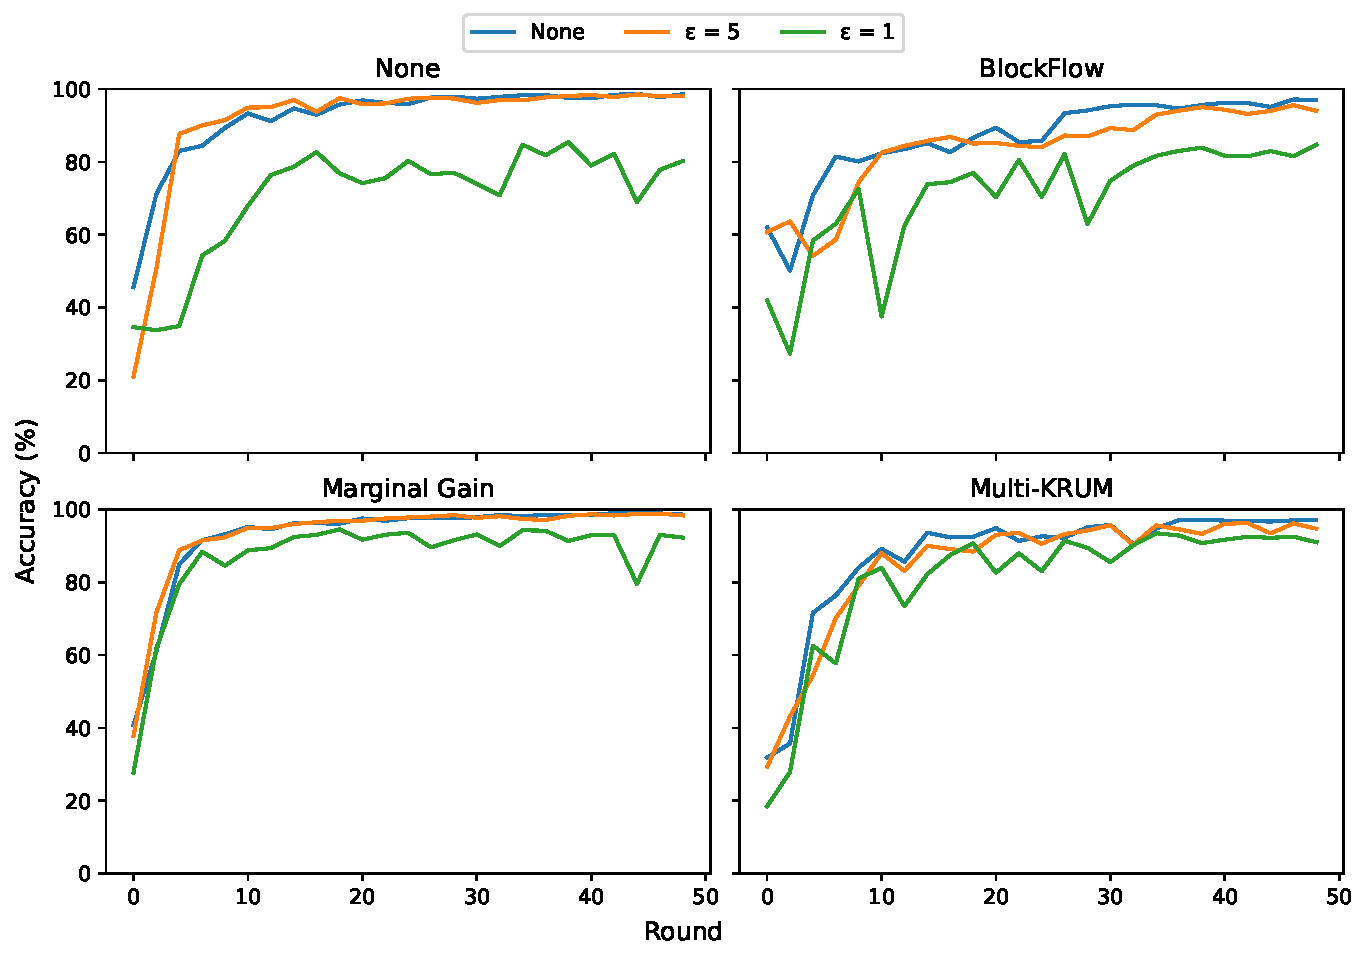
\includegraphics[width=\textwidth]{graphics/privacy/accuracy.pdf}
    \caption{Accuracy Per Privacy Degree}
    \label{fig:accuracy_privacy}
\end{figure}

\section{Accuracy and Convergence}

When it comes to accuracy, different scoring mechanisms have different resistances against the degree of privacy. This can be seen in \autoref{fig:accuracy_privacy}.

On one side of the spectrum, we visualize that not using a scoring mechanism performs the worse with the higher degree of privacy, that is, $\epsilon = 1$. In addition, a lower degree of privacy, $\epsilon = 5$, yields similar results to not using a privacy mechanism at all. The higher the degree of privacy, the higher the noise values that are added to the original weights. Since the weights have added noise, it is expected that the accuracy upon aggregation will be lower the higher the degree of privacy.

Out of the three scoring mechanisms, Marginal Gain and Multi-KRUM perform the best with higher degrees of privacy. As explained in \Cref{background:scoring}, both of these techniques discard the worst updates. In contrast, BlockFlow does not. By discarding the worst submissions according to their scoring algorithm, these techniques always keep the updates that provide the higher accuracy, even after being added noise. Therefore, Multi-KRUM and Marginal Gain have a higher resiliency towards higher privacy degrees, allowing them to maintain high accuracies while preserving privacy.

\section{Communication Costs}

In terms of communication costs, depicted in \autoref{fig:net_privacy}, there are no significant differences depending on the privacy degree we use. Adding noise to the weights does not necessarily increase their sizes and, for that reason, the network traffic costs are not expected to change significantly.

\begin{figure}[!h]
    \centering
    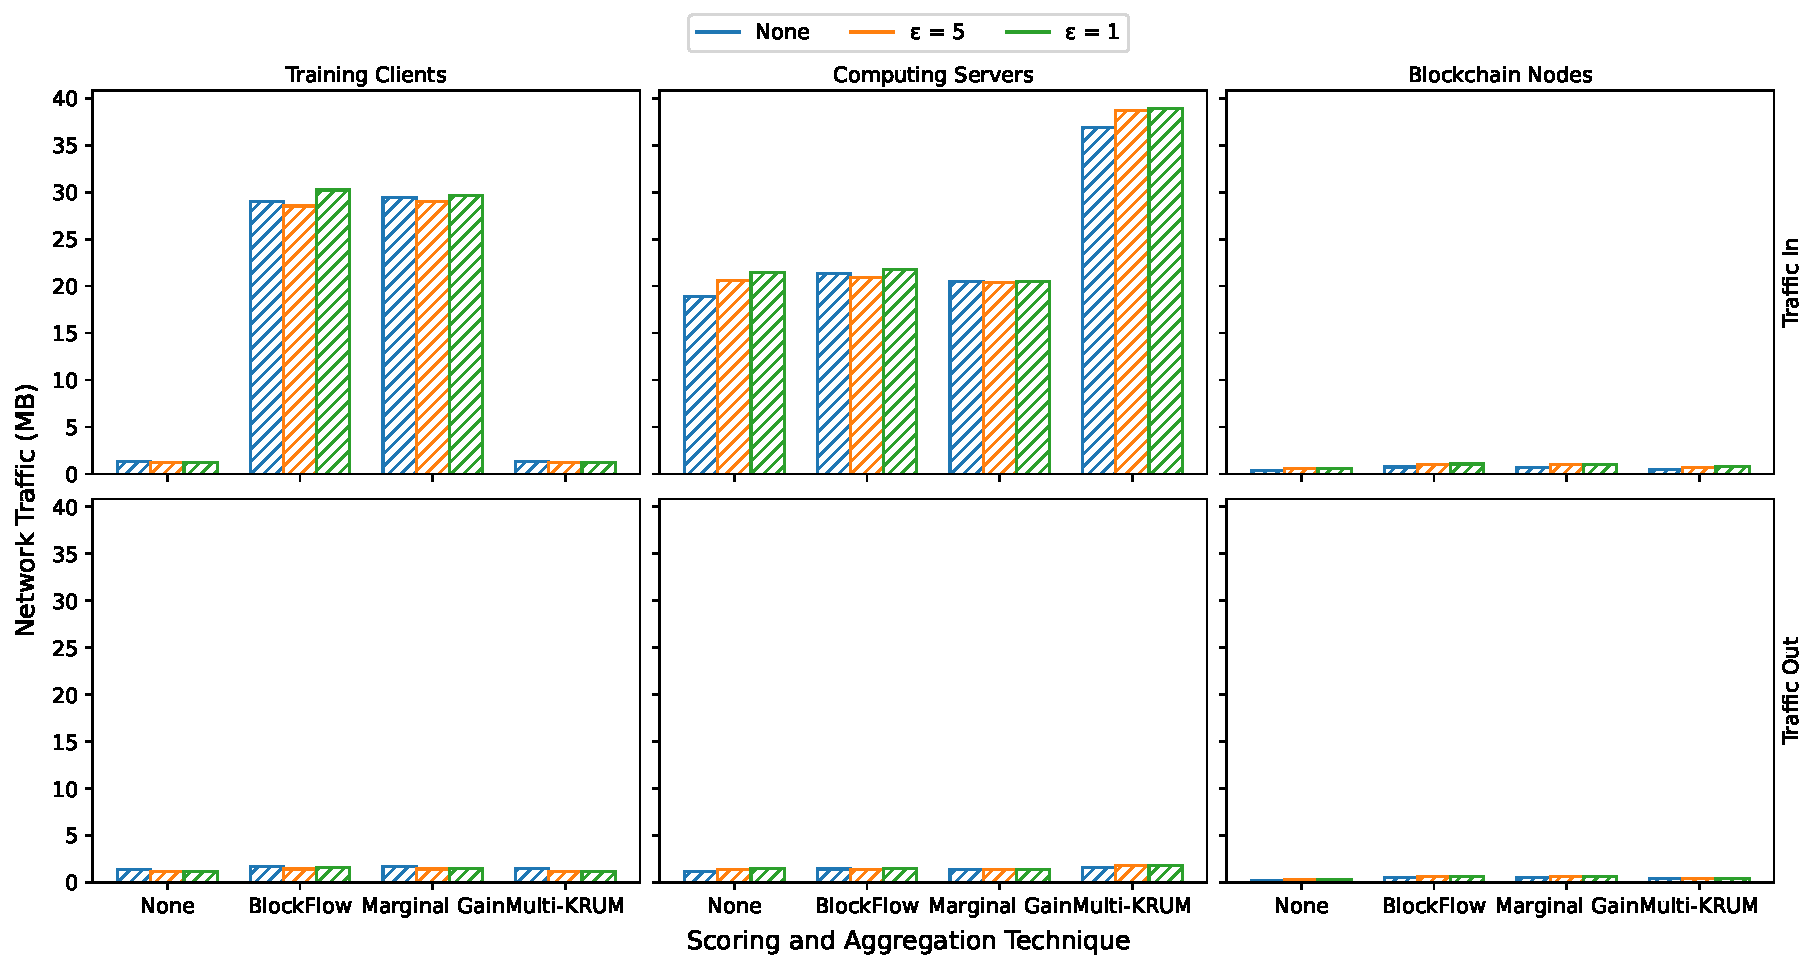
\includegraphics[width=\textwidth]{graphics/privacy/traffic.pdf}
    \caption{Network Traffic Per Privacy Degree}
    \label{fig:net_privacy}
\end{figure}

\section{Computation Costs}

Finally, we look into the computation costs, that is, the RAM and CPU usage across the different types of devices. Since these require a large amount of plots, they are located at the end of the chapter. The privacy mechanisms should only impact the clients, as those are the ones applying the algorithms to their own weights. Therefore, any resource consumption changes should only be visualized in the clients.

As can be seen in \autoref{fig:ram_privacy_clients}, the privacy mechanisms have no significant impact on RAM usage. The mechanism has little to no RAM consumption when compared to the total required for the training process. In contrast, the CPU usage is higher, not necessarily by usage percentage, but by longer usage times. This can be seen in \autoref{fig:cpu_privacy_clients} and is explained by the execution of the privacy mechanism.

As aforementioned, there are no expected changes in RAM or CPU usage at the servers or blockchain nodes.  The only difference presented at the remaining devices, servers and blockchain nodes, is that the process took longer to complete since they had to wait for the clients to train and process the weights, which takes longer. This can be visualized in the remaining plots.

\section{Conclusions}

In conclusion, we have seen that using privacy mechanisms increases the computation costs, and therefore, the resource consumption, at the training clients. This leads to longer mean round execution times as each client has to process their weights and add noise. Consequently, there is a clear trade-off between execution time and privacy. However, increasing the privacy degree does not increase the time.

In addition, we visualized that increasing a privacy degree leads to lower accuracy. This is expected since the privacy mechanisms used introduce noise in the weights. However, some of the scoring mechanisms have a higher resiliency and are able to still achieve higher accuracy values even with high privacy degrees. This is the case of Marginal Gain and Multi-KRUM, which are the most well-performing algorithms.

Finally, we can argue that adding a privacy preserving mechanism to a Blockchain-based Federated Learning system is crucial, specially if the model is trained on sensitive data. One of the main arguments to apply blockchain to a Federated Learning system is the traceability and auditability. To do so, the weights, or their representation in our case, are recorded in the blockchain. This leads to the conclusion that there is a trade-off between traceability and auditability and the requirement for privacy mechanisms, which in turn lead to higher resource consumption.

\clearpage

\begin{figure}[!h]
    \centering
    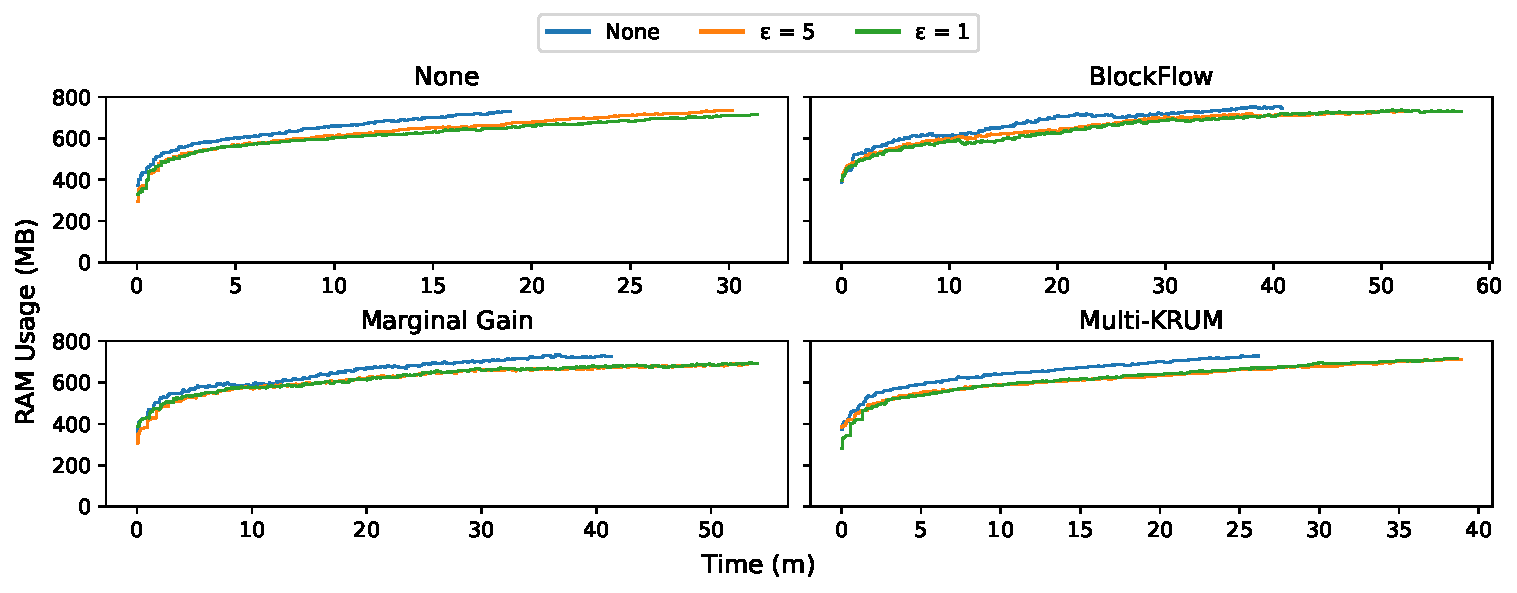
\includegraphics[width=\textwidth]{graphics/privacy/ram_client.pdf}
    \caption{RAM Usage on Training Clients Per Privacy Degree}
    \label{fig:ram_privacy_clients}
\end{figure}

\vfill

\begin{figure}[!h]
    \centering
    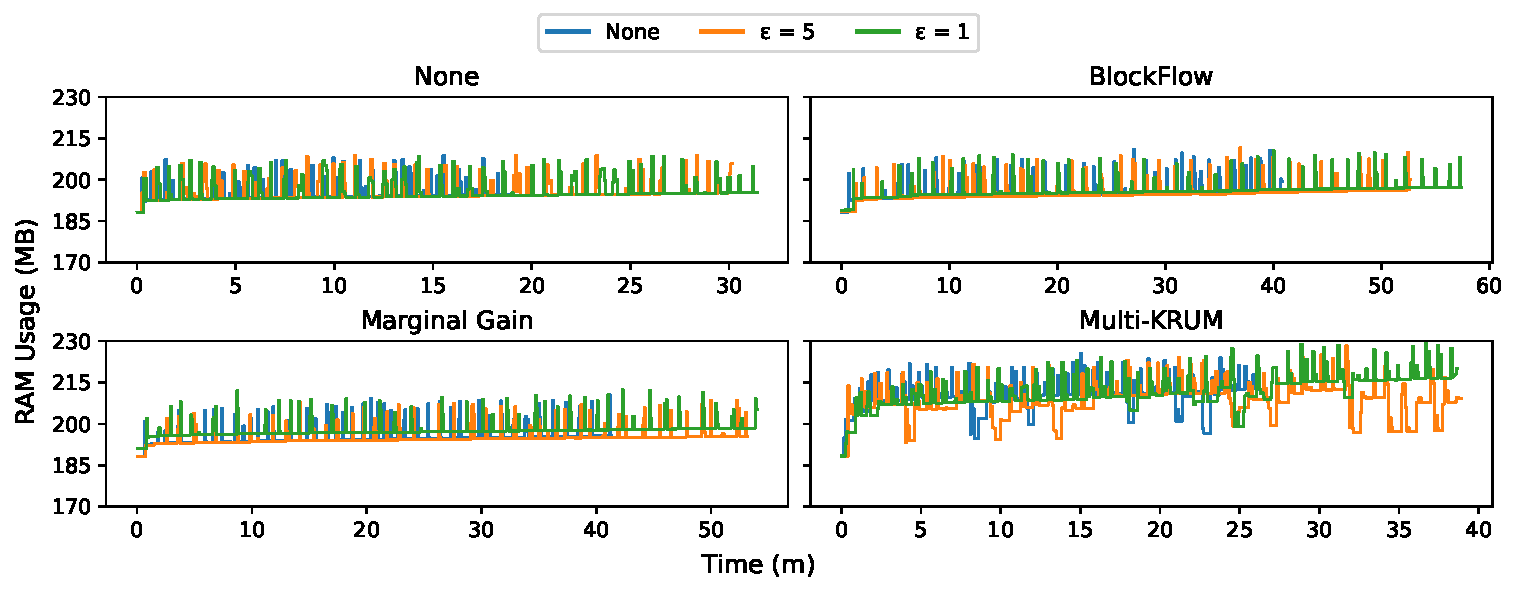
\includegraphics[width=\textwidth]{graphics/privacy/ram_server.pdf}
    \caption{RAM Usage on Computing Servers Per Privacy Degree}
    \label{fig:ram_privacy_servers}
\end{figure}

\vfill

\begin{figure}[!h]
    \centering
    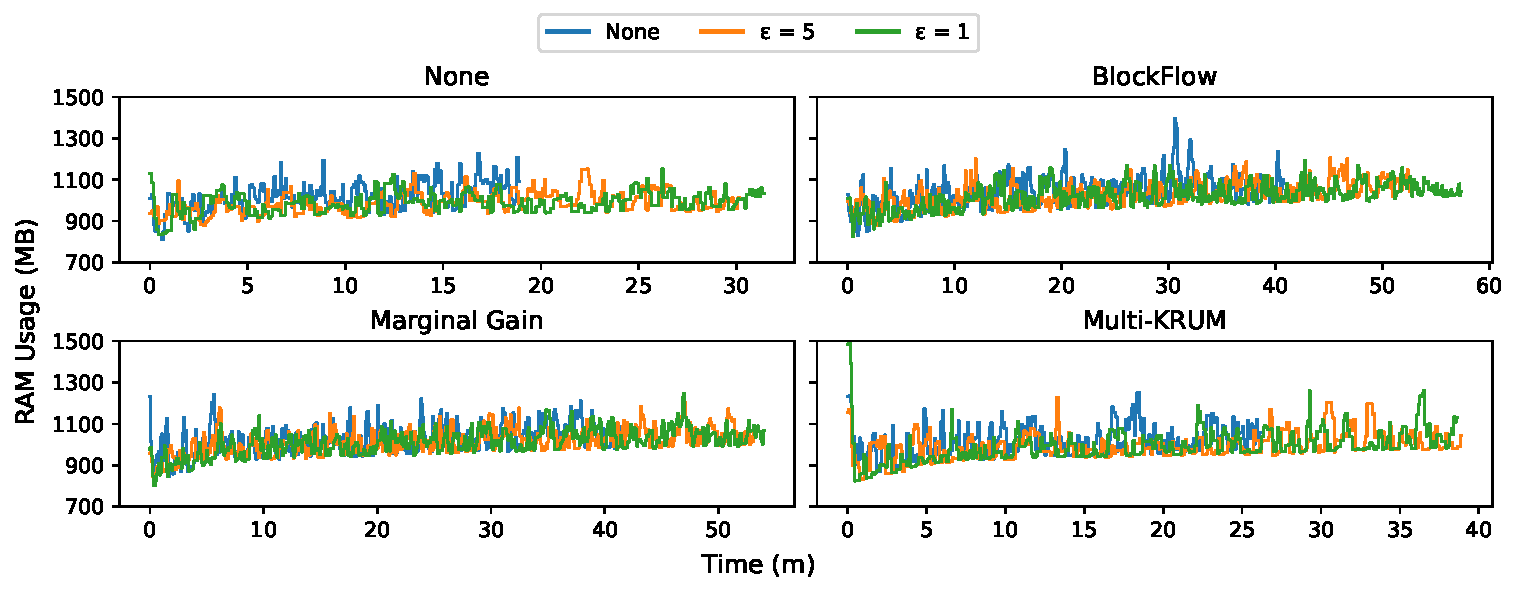
\includegraphics[width=\textwidth]{graphics/privacy/ram_miner.pdf}
    \caption{RAM Usage on Training Clients Per Privacy Degree}
    \label{fig:ram_privacy_miners}
\end{figure}

\clearpage

\begin{figure}[!h]
    \centering
    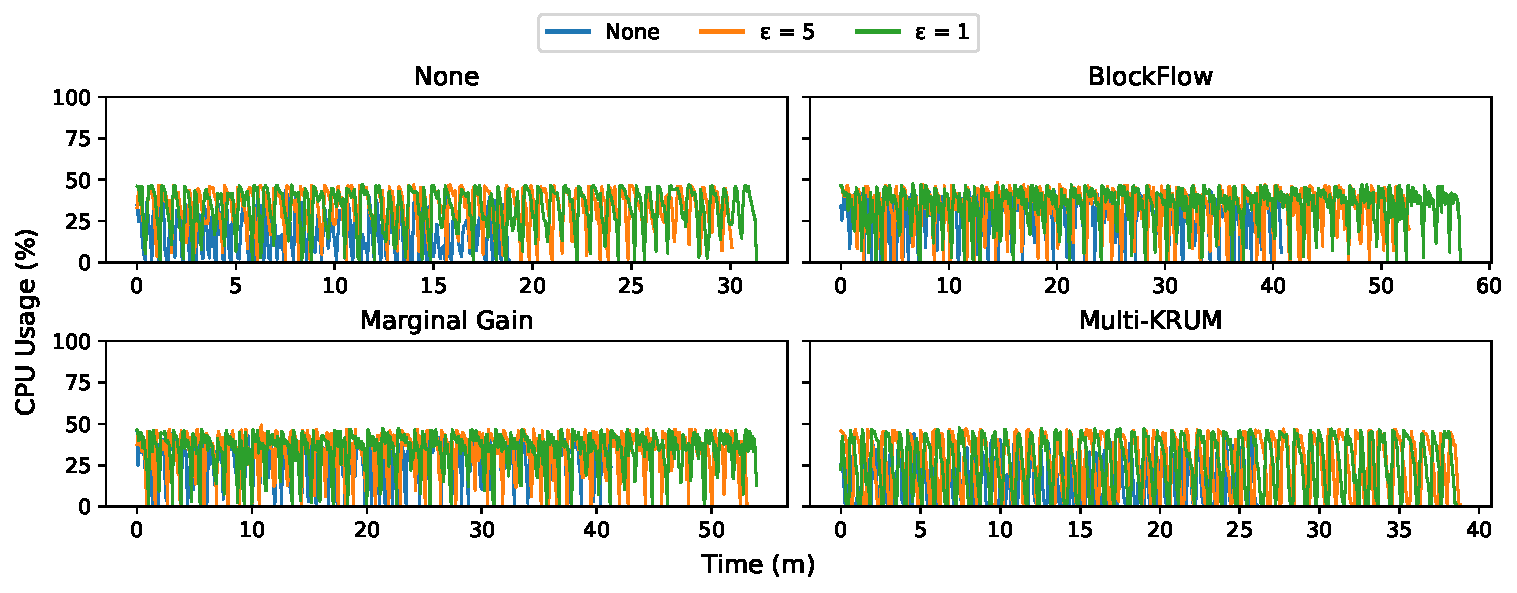
\includegraphics[width=\textwidth]{graphics/privacy/cpu_client.pdf}
    \caption{CPU Usage on Training Clients Per Privacy Degree}
    \label{fig:cpu_privacy_clients}
\end{figure}

\vfill

\begin{figure}[!h]
    \centering
    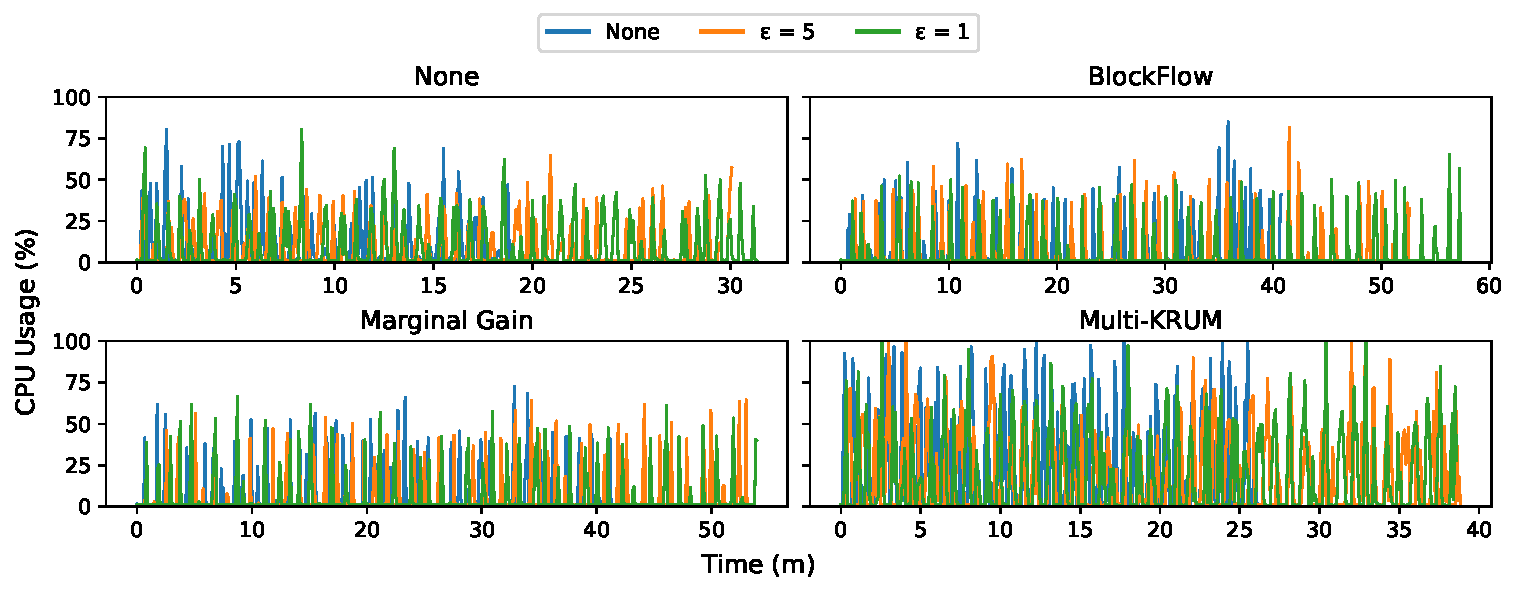
\includegraphics[width=\textwidth]{graphics/privacy/cpu_server.pdf}
    \caption{CPU Usage on Computing Servers Per Privacy Degree}
    \label{fig:cpu_privacy_servers}
\end{figure}

\vfill

\begin{figure}[!h]
    \centering
    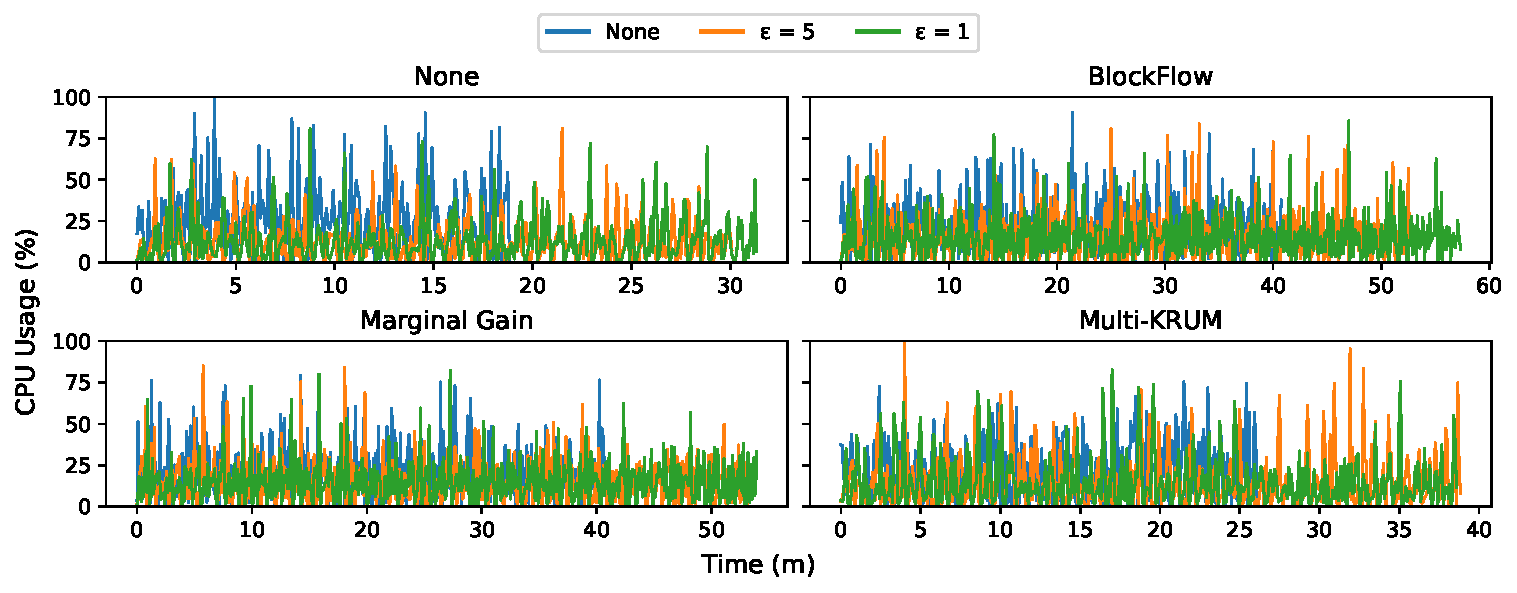
\includegraphics[width=\textwidth]{graphics/privacy/cpu_miner.pdf}
    \caption{CPU Usage on Blockchain Nodes Per Privacy Degree}
    \label{fig:cpu_privacy_miners}
\end{figure}

